% *** Need to put back in all the references to later sections ***

\section{Base model construction}
\subsection{Platform for infectious disease dynamics simulation}

We developed a deterministic compartmental model of COVID-19 transmission using the AuTuMN platform,
publicly available at https://github.com/monash-emu/AuTuMN/.
Our repository allows for the rapid and robust creation and stratification of models of infectious disease epidemiology
and includes pluggable modules to simulate heterogeneous population mixing, demographic processes, multiple circulating
pathogen strains, repeated stratification and other dynamics relevant to infectious disease transmission.
The platform was created to simulate TB dynamics, being an infectious disease whose epidemiology differs markedly
by setting, such that considerable flexibility is desirable \cite{RN58}.
We have progressively developed the structures of our platform over recent years,
and further adapted it to be sufficiently flexible
to permit simulation of other infectious diseases for the purpose of this project.

\subsection{Base COVID-19 model}
Using the base framework of an SEIR model (susceptible, exposed, infectious, removed), we split the exposed and infectious compartments into two sequential compartments each (SEEIIR). The two sequential exposed compartments represent the non-infectious and infectious phases of the incubation period, with the latter representing the ``presymptomatic" phase such that infectiousness occurs during three of the six sequential phases. For this reason, ``active" is a more accurate term for the two sequential ``I" compartments and is preferred henceforward. The two infectious compartments represent early and late phases of active disease, during which symptoms occur if the disease episode is symptomatic, and allow explicit representation of notification, case isolation, hospitalisation and admission to ICU. The ``active" compartment also includes some persons who remain asymptomatic throughout their disease episode, such that these compartments do not map directly to either persons who are infectious or those who are symptomatic (Figure \ref{fig:seeiir}).

\begin{figure}[h]
    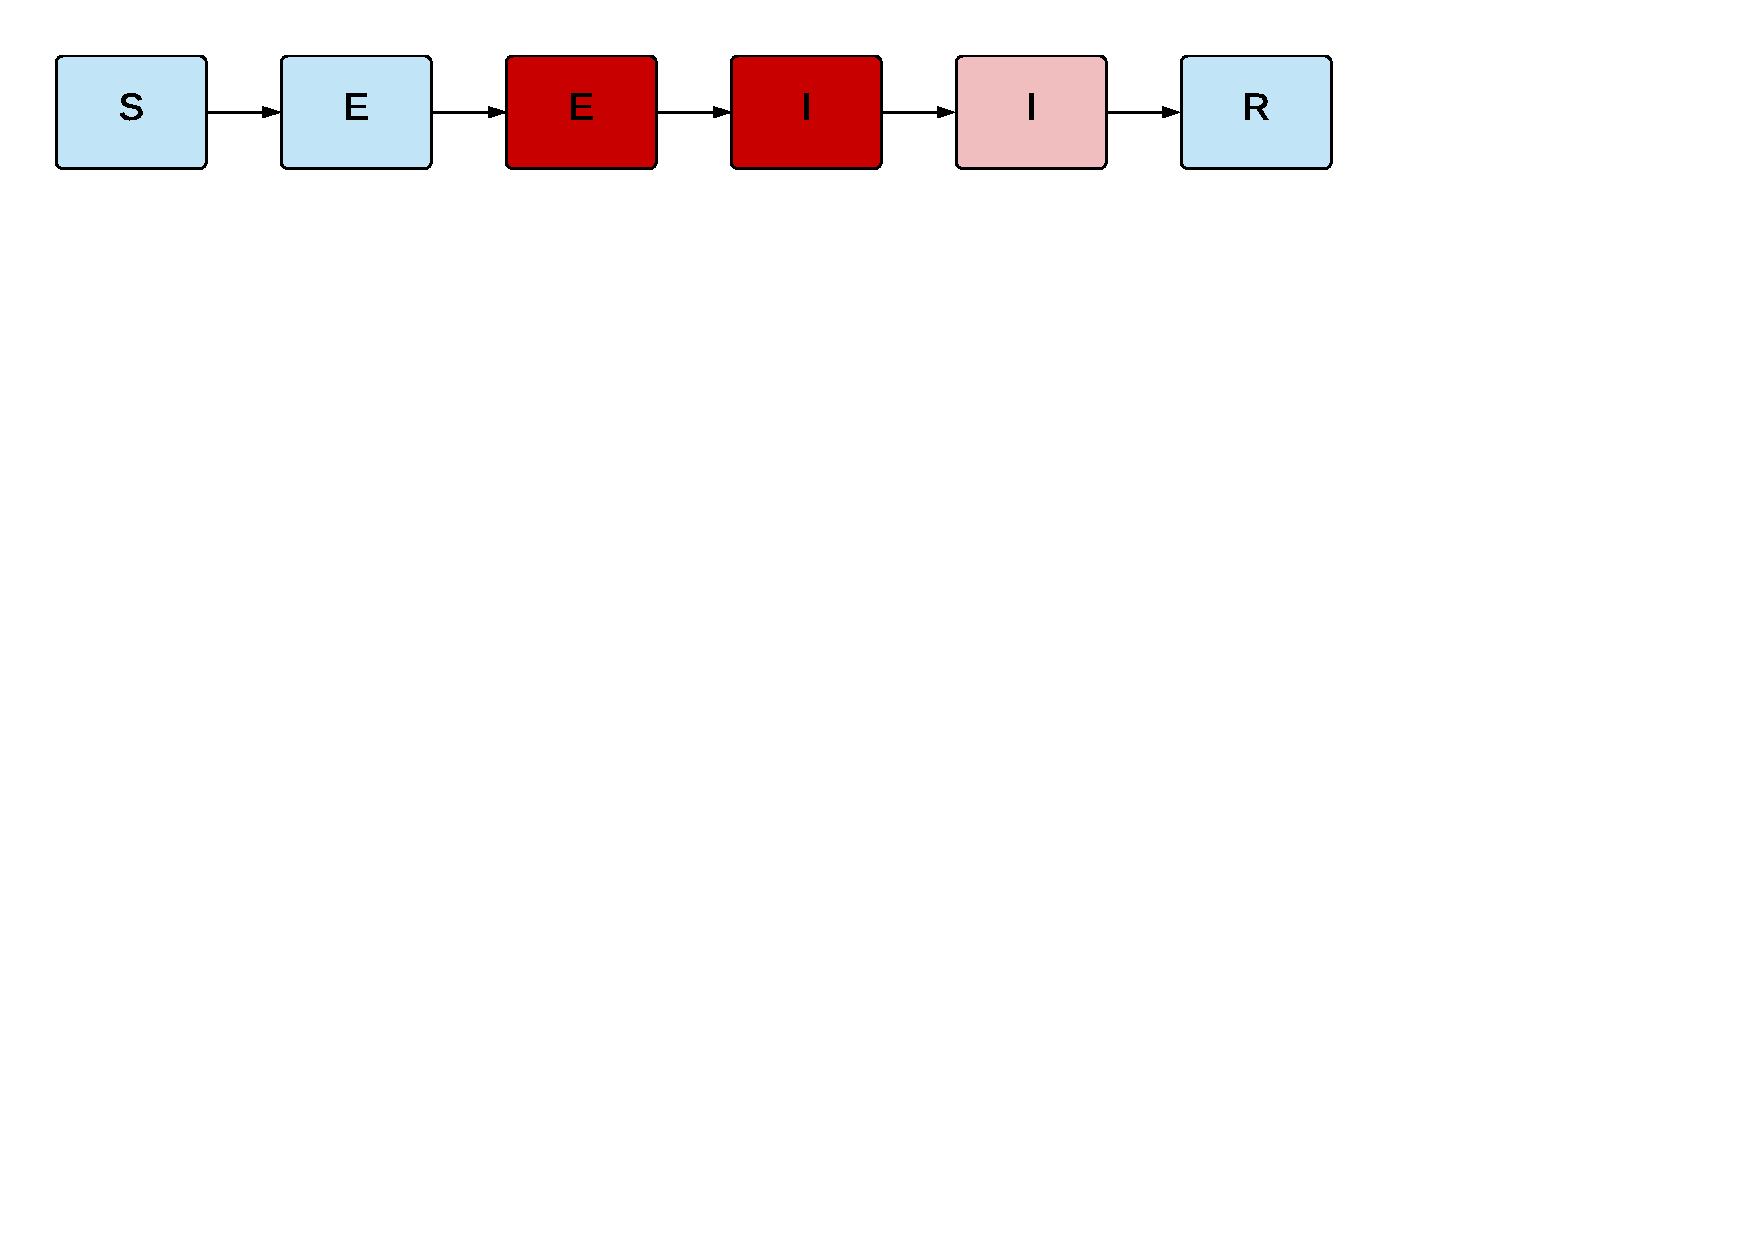
\includegraphics[width=\textwidth]{../model/covid_19_seeiir.pdf}
    \caption{Unstratified compartmental model structure. S = susceptible, E = exposed, I = active, R = recovered/removed. Depth of pink/red shading indicates the infectiousness of the compartment.}
    \label{fig:seeiir}
\end{figure}

The latently infected and infectious presymptomatic periods together comprise the incubation period, with the incubation period and the proportion of this period for which patients are infectious defined by input parameters described below. In general, two sequential compartments can be used to form a gamma-distributed profile of transition to infectiousness following exposure if the progression rates for these two compartments are equal, although in implementing this model the relative sojourn times in the two sequential compartments usually differed. Nevertheless, the profiles implemented are broadly consistent with the empirically observed log-normal distribution of individual incubation periods \cite{RN51}.

The transition from early active to late active represents the point at which patients are detected (for those persons for whom detection does eventually occur) and isolation then occurs from this point forward (i.e. applies during the late disease phase only. This transition point is also intended to represent the point of admission to hospital or transition from hospital ward to intensive care for patients for whom this occurs.

\subsection{Age stratification}
All compartments of this base compartmental structure were stratified by age into five-year bands from 0-4 years of age through to 70-74 years of age, with the final age group being those aged 75 years and older. Heterogeneous baseline contact patterns by age were incorporated using age-specific contact rates estimated by Prem et al. 2017 \cite{RN56}, who combined survey response data with information on national demographic characteristics to produce age-structured mixing matrices with these age groupings. These are then modified by non-pharmaceutical interventions. Our modelled age groups were chosen to match these mixing matrices. The automatic demographic features of AuTuMN that can be used to simulate births, ageing and deaths were not implemented, because the issues considered pertain to the short- to medium-term and the immediate implementation of control strategies, for which population demographics are less relevant.

\subsection{Clinical stratification} \label{clin}
The age-stratified late exposed/incubation and both the early and late active disease compartments were further stratified into five ``clinical" categories: \textit{1)} asymptomatic, \textit{2)} symptomatic ambulatory, never detected, \textit{3)} symptomatic ambulatory, ever detected, \textit{4)} ever hospitalised, never critical and \textit{5)} ever critically unwell (Figure \ref{fig:clinical_strat}).
The proportion of new infectious persons entering stratum 1 (asymptomatic) is age-dependent. The proportion of symptomatic patients (strata 2 to 5) ever detected (strata 3 to 5) is set through a parameter that represents the time-varying proportion of all symptomatic patients who are ever detected (the case detection rate). Of those ever symptomatic (strata 2 to 5), a time-constant but age-specific proportion is considered to be hospitalised (entering strata 4 or 5). Of those hospitalised (entering strata 4 or 5), a fixed proportion was considered to be critically unwell (entering stratum 5, Figure \ref{fig:clinical_rationale}).

\begin{figure}[h]
    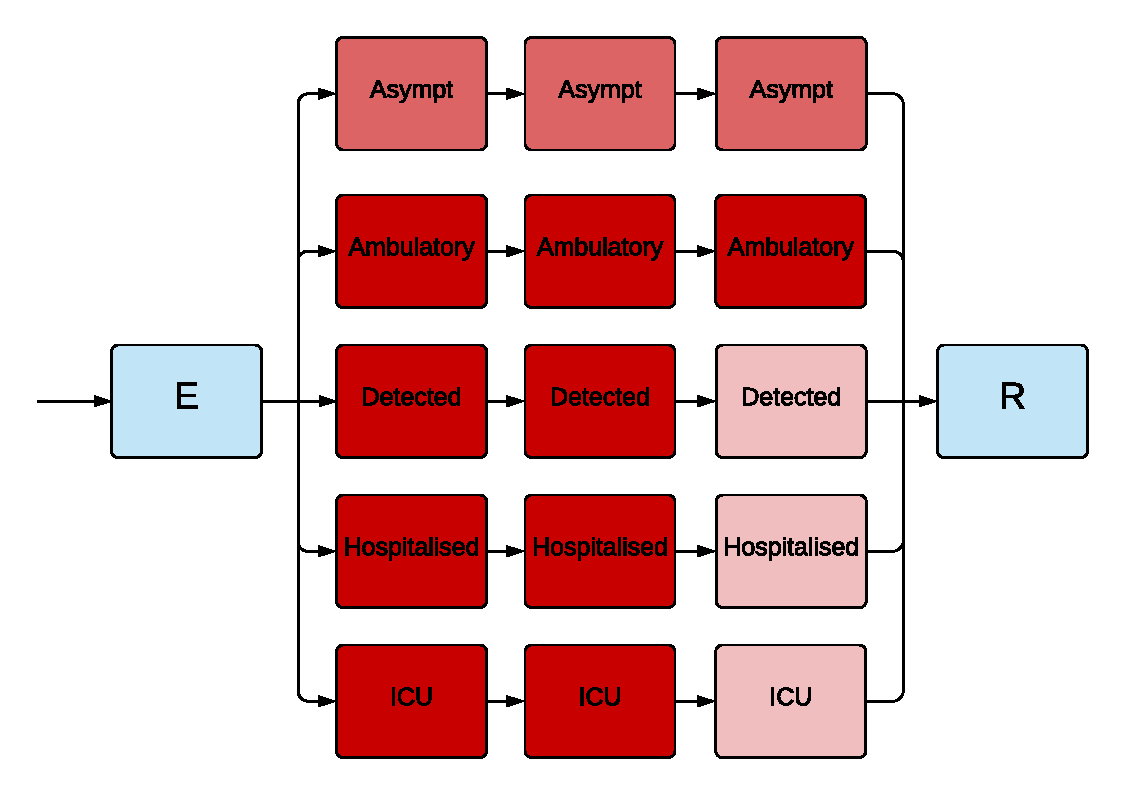
\includegraphics[width=\textwidth]{../model/covid_19_clinical_strat.pdf}
    \caption{Illustration of the implementation of the clinical stratification. Depth of pink/red shading indicates the infectiousness of the compartment. Typical parameter values represented, although the infectiousness of asymptomatic persons is varied in calibration.}
    \label{fig:clinical_strat}
\end{figure}

\begin{figure}[h]
    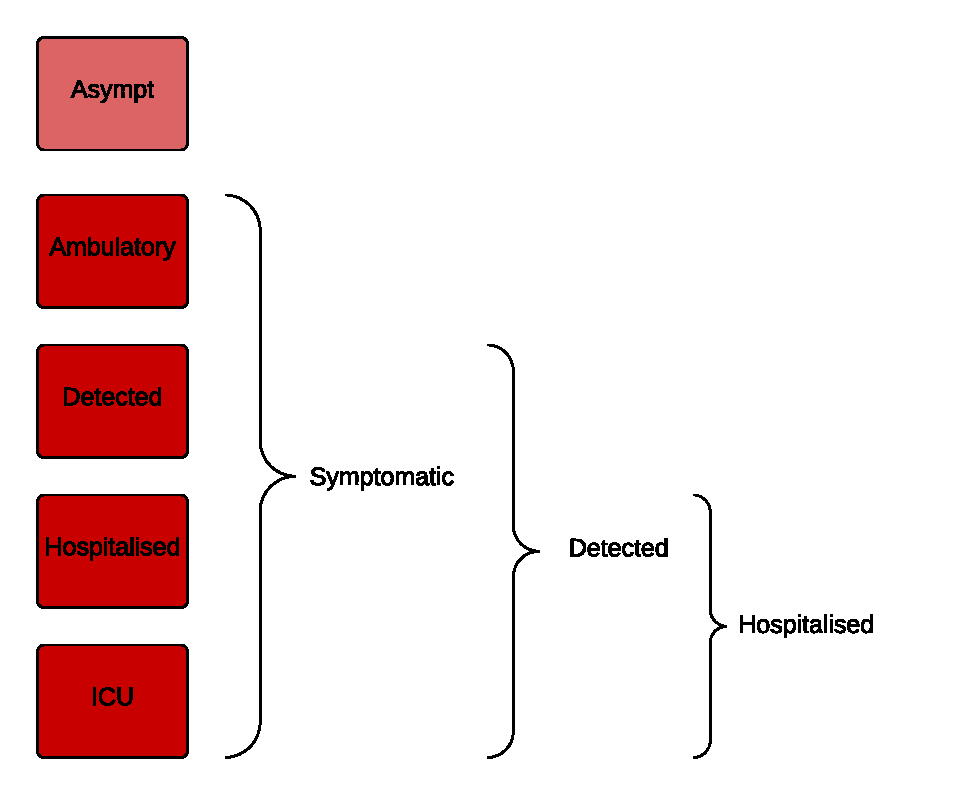
\includegraphics[width=\textwidth]{../model/covid_19_clinical_rationale.pdf}
	\caption{Illustration of the rationale for the clinical stratification.}
    \label{fig:clinical_rationale}
\end{figure}

\subsection{Hospitalisation} \label{hosp}
For COVID-19 patients who are admitted to hospital, the sojourn time in the early and late active compartments is modified, superseding the default values of the sojourn times for these compartments. The point of admission to hospital is considered to be the transition from early to late active disease, such that the sojourn time in the late disease represents the period of time admitted to hospital. For patients admitted to ICU, admission to ICU occurs at this same transition point. For this group, the period of time hospitalised prior to ICU admission is estimated as a proportion of the early active period, such that the early active period represents both the period ambulatory in the community and the period in hospital prior to ICU admission.

\subsection{Infectiousness} \label{infect}
Asymptomatic persons are assumed to be less infectious per unit time active than symptomatic persons not undergoing case isolation (typically by around 50\%, although this is varied in calibration/uncertainty analysis). Infectiousness is also decreased for persons who have been detected to reflect case isolation, and for those admitted to hospital or ICU to reflect infection control procedures (by 80\% for both groups). Presymptomatic individuals are presumed to have equivalent infectiousness to those with early active COVID-19.

\subsection{Application of COVID-19-related death}
Age-specific infection fatality rates (IFRs) were applied and distributed across strata 4 and 5, with no deaths typically applied to the first three strata. A ceiling of 50\% is set on the proportion of those admitted to ICU (entering stratum 5) who die. If the infection fatality rate is greater than this ceiling, the proportion of critically unwell persons dying was set to 50\%, with the remainder of the infection fatality rate then applied to the hospitalised proportion. Otherwise, if the infection fatality rate is less than half of the absolute proportion of persons critically unwell, the infection fatality rate is applied entirely through stratum 5 (such that the proportion of critically unwell persons dying in that age group becomes \textless 50\% and the proportion of stratum 4 dying is set to zero). In the event that the infection fatality rate for an age group is greater than the total proportion hospitalised (which is unusual, but could occur for the oldest age group under certain parameter configurations), the remaining deaths are assigned to the asymptomatic stratum. This approach was adopted for computational ease and is valid because the duration active for persons entering this stratum is the same as for the other non-hospitalised strata, such that the dynamics are identical to assigning the deaths to any of the first three strata. We used the age-specific IFRs previously estimated from age-specific death data from 45 countries and results from national-level seroprevalence surveys \cite{RN54}. We allowed IFRs to vary around the previously published point estimates in order to incorporate uncertainty and to allow the IFRs to differ from the settings in which they were estimated (see Calibration section).
